\documentclass[conference]{IEEEtran}
\IEEEoverridecommandlockouts
% The preceding line is only needed to identify funding in the first footnote. If that is unneeded, please comment it out.
\usepackage{cite}
\usepackage{amsmath,amssymb,amsfonts}
\usepackage{algorithmic}
\usepackage{graphicx}
\usepackage{textcomp}
\usepackage{xcolor}
\usepackage[utf8]{inputenc}
\usepackage[T1]{fontenc}
\def\BibTeX{{\rm B\kern-.05em{\sc i\kern-.025em b}\kern-.08em
    T\kern-.1667em\lower.7ex\hbox{E}\kern-.125emX}}
\begin{document}

\title{Simulação de Desastre - Sistema Multiagentes  Trabalho de IA\\
}

\author{\IEEEauthorblockN{Lucas Vieira, Lucas Martins, Victor Henrique Ribeiro}
\IEEEauthorblockA{\textit{UNESP Júlio de Mesquita Filho} \\
\textit{ Ciência da Computação Noturno, 2018}\\
Rio Claro, Brasil\\}
}

\maketitle

\begin{abstract}
Um breve estudo sobre uma ferramenta de simulação de desastre, e programação de multiagentes
\end{abstract}

\begin{IEEEkeywords}
RescueCup, Multiagentes, Inteligência Artificial, Simulação.
\end{IEEEkeywords}

\section{Introdução}
A Inteligência Artificial que consiste em a criação de softwares inteligentes, que tem a capacidade simular a capacidade humana de raciocinar, tomar decisões e resolver problemas . Suas aplicações são muitas, e aqui iremos ver uma aplicação de simulação de desastre, que consiste em montar a melhor estratégia, programaticamente para atuar em uma situação de desastre.

\section{Ferramentas}

\subsection{Robocup Rescue Simulation Server}

Este software trata-se do centro do nosso estudo, onde os vários simuladores comunicam entre-si e fazem a comunicação entre agentes tudo através de um simulador de Kernel do próprio simulador que gerencia toda essa interação.

\begin{figure}[htbp]
\centerline{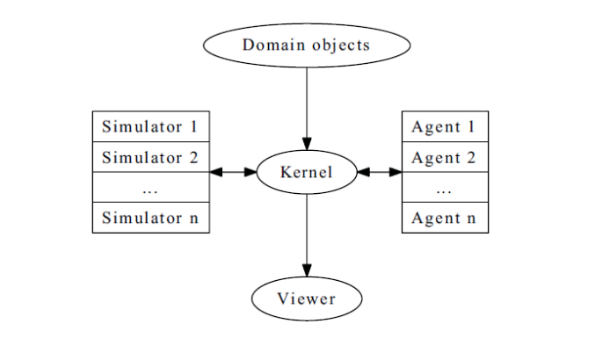
\includegraphics[scale=0.3]{fig1.png}}
\caption{RoboCup Rescue Agent Simulation platform architecture \cite{b1}}
\label{fig}
\end{figure}

A composição do server é entre 6 simuladores:
\begin{itemize}
\item \textit {Clear Simulator} - Responsável pela remoção de bloqueios das estradas. 
\item \textit {Collapse Simulator} - Responsável por gerenciar os danos estruturais dos prédios para criar bloqueios.
\item \textit {Ignition Simulator} - Realiza o princípio de incêndio nos prédios durante a simulação.
\item \textit {Fire Simulator} - Responsável por espalhar o fogo entre os edifícios.
\item \textit {Traffic Simulator} - Simulador responsável pelo movimento das entidades humanas.
\item \textit {Misc Simulator} - Responsável pelo dano de humanos e estruturas.
\end{itemize}

Na arquitetura do ambiente, como visto na Fig 1, ainda estão os objetos da cena, que estão dispostos em um arquivo ponto .gml, onde estão todas as estruturas e vias do mapa. O "Viewer" seria uma visualização gráfica do sistema, onde estão sendo atualizados os agentes e estruturas no ambiente. 

Já os agentes são responsáveis pelas ações que alteram o ambiente, onde enviam ações para o kernel, ele gerencia a comunicação com o determinado simulador responsável pela ação e atualiza o "Viewer" de acordo com a situação atual do ambiente, mais detalhes serão explicados na seção sobres os Agentes e o ambiente.
\subsection{Eclipse - Linguagem Java}
A própria ferramenta tem bibliotecas e samples são todas feitas em Java, portanto foi facilmente a linguagem escolhida para o trabalho. No Robocup Rescue a atuação das equipes que participam do evento é na formulação de estratégias entre os agentes e de agentes com o ambiente. Portanto o desafio é gerenciar todas essas variantes programaticamente. 
O código é composto de classes auxiliares e classes do código dos Agentes. A função do eclipse é compilar este código e carregar os agentes ao Simulation Server, onde após isso os algoritmos serão executados no kernel do simulador, por fim atuando na simulação.

\subsection{JOSM Editor}
\textit {JOSM Editor - Java OpenStreetMap Editor} é a ferramenta utilizada para criar o nosso ambiente,que é o mapa que contém prédios e vias.É uma ferramenta de software livre, onde é possivel selecionar uma área em qualquer lugar mapa-mundi e é feita a classificação dos objetos em uma área.

\begin{figure}[htbp]
\centerline{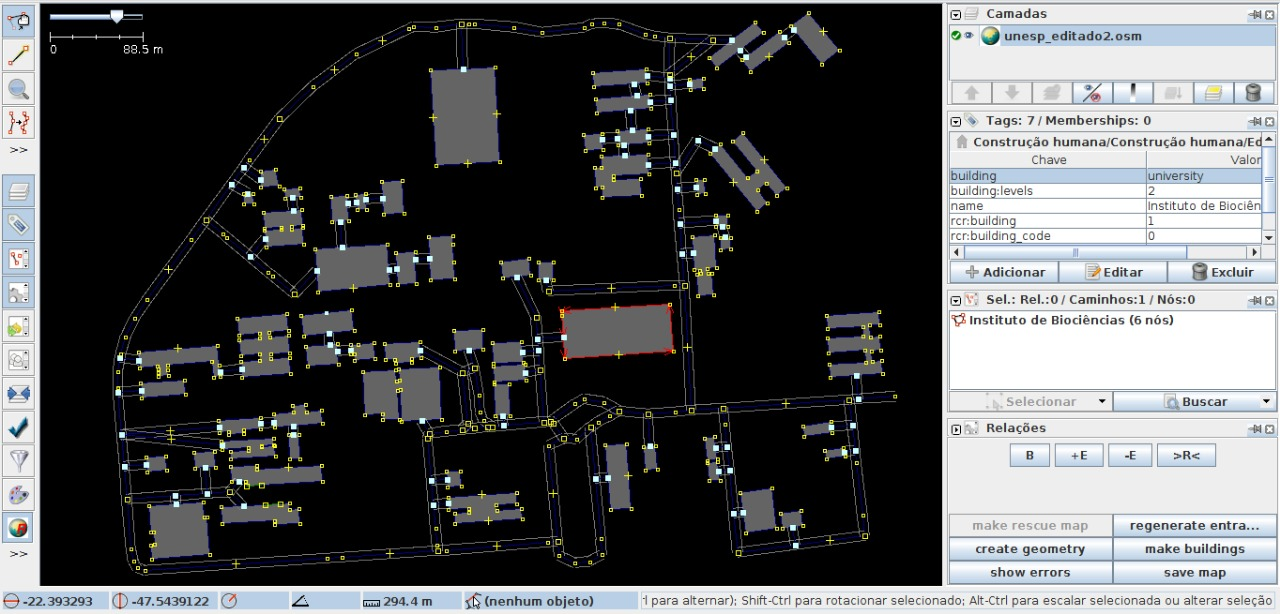
\includegraphics[height=3.3cm]{fig3.jpeg}}
\caption{Imagem do mapa da UNESP criado pelo JOSM \cite{b2}}
\label{fig}
\end{figure}

No nosso projeto, utilizamos a ferramenta para criar um mapa da UNESP Júlio de Mesquita Filho como mostrado na Figura 2, onde tivemos que retirar muitos detalhes do mapa, para que o Simulation Server utilize corretamente os objetos do mapa.

\section{Ambiente - Entidades do Ambiente}
O ambiente é o lugar onde os agentes e simuladores interagem, onde ocorre a simulação. E que no caso deste projeto é representado por um mapa, onde há localizações, edifícios e vias.
\subsection{Blockade}
Blockades ou bloqueios são entidades que obstruem caminhos nas vias, portanto dificultando a movimentação dos agentes.
Eles são gerados pelo \textit{Collapse Simulator} de acordo com o dano aos edifícios, simulando assim detritos e prédios entrando em colapso em uma situação de desastre. Os bloqueios possuem certas propriedades como: posição, custo de reparo, formato, coordenadas e ápice.

\subsection{Área}
Áreas são considerados os prédios e ruas do mapa, os bloqueios acontecem em ambos, mas somente nas ruas os bloqueios são visíveis. Programaticamente as áreas possuem certas propriedades,como: bloqueios na área, arestas da área, lista de áreas vizinhas e coordenadas da área no mapa.
\subsection{Buildings - Localizações Chave}
Há quatro localizações chave no simulador, e essas são:
\begin{itemize}
\item \textit {Refuge} - Refúgio para os civis.
\item \textit {Ambulance Central} - Central de comunicação do ambulance team
\item \textit {Fire Station} - Central de comunicação de Fire brigade
\item \textit {Police Office} - Central de comunicação da Police Force
\end{itemize}
Mais detalhes sobre comunicação serão descritos posteriormente neste documento.


\section{Agentes}
Os agentes são os atores do simulador, que interagem com o sistema e comunicam entre si. Nesta seção serão explicados as ações e funções de cada um.
\subsection{Civillians}
Os civis são os agentes que devem ter seu caminho facilitado por outros agentes até o refúgio.
\subsection{Police Force}
A polícia tem como objetivo limpar os blockades, ou seja, facilitar o caminho de todos os agentes no ambiente.
\subsection{Fire Brigade}
A fire Brigade tem como função apagar incêndios em prédios, eles carregam uma certa quantidade de 'água', que após ser usado deve ser reabastecido em um refuge.
\subsection{Ambulance Team}
Ambulance Teams são os agentes que resgatam outros agentes e levam ao refuge, eles também salvam agentes enterrados e carregam no máximo um agente.
\subsection{Central Agents}
Representados como localizações chave, Ambulance Centers, Fire Stations e Police Offices. Tem como única função realizar a comunicação via rádio com os agentes.

\section{Percepção e Comunicação}

\subsection{Percepção - Lines of sight}
A percepção de cada agente é representada por linhas no simulador, ou seja, aonde as linhas conseguem atingir é o que o agente computa o que está acontecendo no ambiente, como representado na Figura 3.
\begin{figure}[htbp]
\centerline{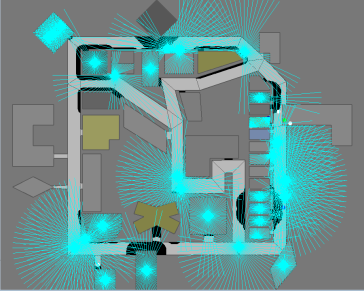
\includegraphics[scale=0.5]{fig2.png}}
\caption{Lines of Sight - Representação das linhas de visões dos agentes \cite{b1}}
\label{fig}
\end{figure}
Por exemplo, se um agente vê um bloqueio e o mesmo sai do seu campo de visão, mesmo se o bloqueio for limpo, para o agente ainda vai haver um bloqueio aonde ele passou. Portanto a sua visão atualiza seu conhecimento do ambiente.

\subsection{Comunicação}
A comunicação auxilia na tomada de ações dos agentes, atualizando as percepções de mundo entre agentes.

Existem dois tipo de comunicação no simulador:
\begin{itemize}
\item \textit {direct communication} - É a simulação de uma comunicação oral humana,portanto é emitida de um agente e outro agente só a recebe se estiver dentro do raio de alcance do emissor.
\item \textit {radio communication} - comunicação por radio realiza a interação das localizações chave para com os agentes, portanto ela atinge todos os agentes de uma mesma classe por todo o mapa.
\end{itemize}

Ambos os tipos de comunicação estão suscetíveis a falhas, mas no caso do radio communication, há duas falhas possíveis, em ambos os casos há a possibilidade de \textit{dropout} que é a a falha de um agente em receber a mensagem. E a outra falha possível seria a de \textit{failure}, que ocorre no caso do radio apenas, onde um agente recebe a mensagem mas ela vem vazia.

\section{Programação de Agentes}
A programação de agentes envolve a utilização de conceitos que imitam a atuação humana em situações de desastre. Por exemplo, ouvir algum civil pedindo por socorro, envolve passar informações valiosas para agir no ambiente para outros agentes. E principalmente agir em prol do objetivo, que é o resgate de civis.
Lembrando que os agentes só podem realizar uma ação por 'turno', seja essa andar, resgatar, etc. Já a comunicação é permitida que seja uma ação adicional, portanto pode se mover e se comunicar em um 'turno', por exemplo.
\subsection{Civis}
Os civis tem o código provido pelo próprio simulador, eles traçam um caminho para o refúgio, se esse caminho tiver obstruído ele espera por socorro. Ele também chama por socorro para agentes a sua volta receberem a sua posição.
\subsection{Police Force}
Esse agente age mediante a 3 estados: \textit{AVAILABLE}(Disponível), \textit{WALK}(Andando) e \textit{CLEAR}(Limpar). A principal função de um policial é limpar as vias do ambiente, portanto foi priorizado o agente estar se movendo sempre que disponível, com o objetivo de encontrar mais blockades para limpar.

Na ação \textit{WALK}, o agente anda de 2 formas, uma seria randomicamente, através de uma função que procura caminhos possíveis e sorteia um para o agente andar, assim encontrando possíveis blockades. A outra forma de andar seria direcionada a um objetivo, que no caso do policial seria um blockade, dessa maneira quando é encontrado um bloqueio, e o agente entra em estado \textit{CLEAR}, o mesmo vai andar em direção ao bloqueio buscando eliminá-lo.

A ação \textit{CLEAR}, que é a principal função do policial, consiste em no momento que for detectado um blockade, o mesmo deve ser limpo com a função sendClear(), que com o envio das informações do blockade, realiza a limpeza do bloqueio. A complexidade dos bloqueios é algo definido pelo o simulador 'collapse', portanto o sendClear(), que utiliza o simulador 'clear', devido a complexidade do bloqueio a limpeza, não é instantânea, pode necessitar de várias chamadas da função sendClear() para eliminar um blockade.
\subsection{Ambulance Team}

\subsection{Fire brigade}

\begin{thebibliography}{00}
\bibitem{b1} Annibal B. M. da Silva, Luis G. Nardin and Jaime S. Sichman, ``Robocup Rescue Simulator Tutorial,'' Laboratório de Técnicas Inteligentes - Escola Politécnica da USP, São Paulo - SP.
\bibitem{b2} Alan D. Barroso, Felipe Santana e Victor Lassance, "Tutorial for the Creation of a Robocup Rescue Simulator Map", Escola Politécnica da USP, São Paulo - SP.

\end{thebibliography}

\end{document}
